\chapter{Einführung}
Ein eingettetes System ist in einen technischen Kontext oder Prozess eingebettet.

Im wesentlichen kann ein eingebettetes System als ein Computer, der einen technischen Prozess steuert oder regelt, betrachtet werden.
\todo{Grafik}

\section{Architektur eines Eingebetteten Systems}
\subsection{Eigenschaften eines Eingebetteten Systems}
\begin{itemize}
    \item Enge Verzahnung zwischen Hard- und Software
    \item Strenge funktionale und zeitliche Randbedinungen
    \item Zusätzlich zum Prozessor wird I/O Hard- und Software benötigt
    \item Oftmals wird Anwendungsspezifische Hardware benötigt
\end{itemize}
$\Rightarrow$ Keine \glqq{}General-Purpose\grqq{} Lösung möglich

Zusätzliche Probleme:
\begin{itemize}
    \item Wenig Platz
    \item Nur beschränkte Energiekapazität
    \item System darf nicht warm werden
    \item Kostengünstig
\end{itemize}

\subsection{Zusätzliche Herausforderungen beim Entwurf}
Die Entwicklung eines eingebetteten Systems ist kein reines Software-Problem, zusätzlich muss beachtet werden:
\begin{itemize}
    \item Auswahl eines Prozessors, Signalprozessors, Microcontrollers
    \item Ein-/Ausgabe Konzept\&Komponenten
        \begin{itemize}
            \item Sensoren und Aktoren
            \item Kommunikationsschnittstellen
        \end{itemize}
    \item Speichertechnologien und Anbindung
    \item Systempartitionierung: Aufteilen der Funktionen der Komponente
    \item Logik- und Schaltungsentwurf
    \item Auswahl geeigneter Halbleitertechnologien
    \item Entwicklung von Treibersoftware
    \item Wahl eines Laufzeits-/Betriebssystems
    \item Die eigentliche Softwareentwicklung
\end{itemize}
$\Rightarrow$ Aufteilung des Entwurfs auf mehrer Entwurfsebene

\subsection{Entwurfsebenen}
\begin{table}[H]
    \centering
    \begin{tabular}{p{.25\textwidth}p{.25\textwidth}p{.25\textwidth}p{.25\textwidth}}
        \toprule
        Verhalten & Syntheseschritt & Entscheidungen & Test \\
        \midrule
        System Specification & Systemsynthese & HW/SW/OS & Modelsimulator / Checker \\
        Behavioural Specification & Verhalten / Architektursynthese & Verarbeitungs-einheiten & HW/SW-Simulation \\
        Register-Transfer-Specification & RT-Synthese & Register, Addierer, Mux & HDL-Simulation \\
        Logic-Specification & Logiksynthese & Gatter & Gate-Simulation \\
        \bottomrule
    \end{tabular}
    \caption{Entwurfsebenen}
\end{table}

\todo{Graphik}

\section{Hardwarespezifikationssprachen}
\begin{itemize}
    \item Verilog
    \item VHDL (Very High Speed Integrated Circuit Description Language)
\end{itemize}

\begin{figure}[H]
    \centering
    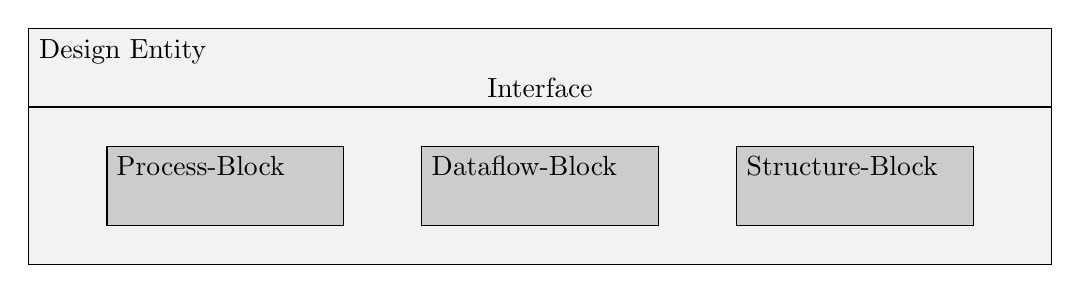
\begin{tikzpicture}
        \filldraw [draw=black,fill=gray!10] (0,0) rectangle (13,3);
        \node at (1.2,2.7) (de){Design Entity};
        \draw (0,2) -- (13,2) node[above,pos=.5] {Interface};
        \filldraw [draw=black,fill=gray!40] (1,0.5) rectangle (4,1.5);
        \filldraw [draw=black,fill=gray!40] (5,0.5) rectangle (8,1.5);
        \filldraw [draw=black,fill=gray!40] (9,0.5) rectangle (12,1.5);
        \node[below right] at (1,1.5) (){Process-Block};
        \node[below right] at (5,1.5) (){Dataflow-Block};
        \node[below right] at (9,1.5) (){Structure-Block};
    \end{tikzpicture}
    \caption{Aufbau einer Design-Entity}
\end{figure}

\paragraph{Process-Block}
Sequentiell abgearbeitete Logik:
\begin{lstlisting}[style=vhdl]
    process(clk)
    begin
        ...
    end
\end{lstlisting}

\paragraph{Dataflow-Block}
Konkurrent abgearbeitete Logik:
\begin{lstlisting}[style=vhdl]
    begin
        ...
    end
\end{lstlisting}

\paragraph{Structure-Block}
Zusammenschalten weiterer Design-Entitys:
\begin{figure}[H]
    \centering
    \includegraphics[width=0.4\textwidth]{structure.pdf}
    \caption{Structure-Block}
\end{figure}

\subsection{Aufbau von VHDL-Beschreibungen}
\begin{itemize}
    \item \lstinline[style=vhdl]{use}: Import von Bibliotheken
    \item \lstinline[style=vhdl]{entity}: Schnittstellenbeschreibung
    \item \lstinline[style=vhdl]{architecture}: Implementierung der Entity
    \item \lstinline[style=vhdl]{configuration}: \lstinline[style=vhdl]{architecture} zu \lstinline[style=vhdl]{entity} auswählen
\end{itemize}

\subsection{Beispiel: Multiplexer}
Entity-Deklaration:
\begin{lstlisting}[style=vhdl]
    entity MUX is
        port(a,b,sel: in Bit;
            f: out Bit);
    end MUX;
\end{lstlisting}

\subsubsection{Als Process-Block}
\begin{lstlisting}[style=vhdl]
    architecture BEHAVIOUR_MUX of MUX is
    begin
        process(a,b,sel)
        begin
            if sel = '1' then f <= a;
            else f <= b;
        end process;
    end BEHAVIOUR_MUX;
\end{lstlisting}

\subsubsection{Als Dataflow-Block}
\begin{lstlisting}[style=vhdl]
    architecture DATAFLOW_MUX of MUX is
    begin
        f <= a when sel = '1' else b;
    end DATAFLOW_MUX;
\end{lstlisting}
alternativ geht auch:
\begin{lstlisting}[style=vhdl]
    architecture DATAFLOW_MUX of MUX is
    begin
        f <= (a and sel) or (b and (not sel));
    end DATAFLOW_MUX;
\end{lstlisting}
eine weitere Option:

\begin{lstlisting}[style=vhdl]
    architecture DATAFLOW_MUX of MUX is
    signal nsel, f1, f2 : Bit;
    begin
        nsel <= not sel;
        f1 <= a and sel;
        f2 <= b and nsel;
        f <= f1 or f2;
    end DATAFLOW_MUX;
\end{lstlisting}
Alternativ: Mit Variablen
